

	
	
	
	Свойства и результаты прочих исследований:
	[Vaganov corrected]

\section{Методы исследования кристалличности}

Тырим описание методов и формулы из \cite{cryst3}
Кристалличность полимеров может быть проанализирована, если обнаружить раличия в характеристиках аморфных и кристаллических областей. Приведем широко используемые методы, с помощью которых определяется кристалличность.

\subsection{Плотность}
The most basic is the
small differences in the density of the crystalline and amorphous regions that makes it
possible to use density measurement for the evaluation of the polymer crystallinity.
При аддитивности по объему:
\[
\%_{x_m} =\frac{\nu - \nu_a}{\nu_c - \nu_a}\cdot100 = \frac{\rho_c}{\rho}\cdot\frac{\rho - \rho_a}{\rho_c-\rho_a}
\]
При аддитивности по массе:
\[
\%_{x_{\nu}} =\frac{\rho - \rho_a}{\rho_c-\rho_a}
\]
Точность измерения < 0.1 кг/м3\\
The density of the crystalline phase
can be calculated from the crystallographic unit cell parameters. The density of
the amorphous phase can be obtained by extrapolating to room temperature the specific
volume of the melt measured at various temperatures by dilatometric methods
[16,17]. The crystalline and the amorphous densities can also be determined experimentally
by extrapolating the densities of a series of samples with known crystallinities
as measured by XRD.\\
Короче нужен будет рса

\subsection{Термический анализ}


Equally fundamental is the thermal characteristics of the crystalline and the amorphous
regions. Because crystalline domains melt upon heating, and amorphous domains do
not, heat of fusion can be a used as a measure of the degree of crystallinity. \\
The amount of energy absorbed
depends on the degree of crystallinity. This energy can be determined using\\
differential scanning calorimetry (DSC). DSC measures the amount of heat absorbed
or released by the sample relative to a reference (an empty pan) as it is taken through
various thermal transitions at a constant heating or cooling rate, and under
isothermal conditions as a function of time.\\
The mass percent crystallinity (xm) of a specimen can be calculated from the
measured heat of fusion (DHm) and the knowledge of the value for 100\% crystalline
material $\Delta H^0_m$
from the relation
\[
\%x_m = \frac{\Delta H_m - \Delta H_c }{\Delta H^0_m}\cdot100
\]
The term DHc is the heat of cold crystallization. A typical DSC scan consists of a heat cool reheat cycle, all three being done at a rate of 10 C/min. Because materials
change during heating as well as upon cooling, the crystallinity should be determined
from the scan obtained during the first heat.\\
The implementation of Eq. (3.5)
into practice to evaluate the crystallinity is not straightforward!!!\\
issues. First, a proper baseline has to be drawn for precise determination of the crystallinity. \\
Second, crystallization of the sample during heating, cold crystallization,
is a serious problem in evaluating the crystallinities of samples with low
levels of crystalline order.\\

\subsection{Спектроскопия}
ИК-спектроскопия, раманоское рассеяние и ЯМР -- три широко испольщуемые спектроскопические методы, используемые для анализа структурных характеристик, таких как конформация, стереорегулярность, ориентация, внутри- и межмолекулярные взаимодействия полимеров. [38] 
Эти техники также используются для определения кристалличности, после калибровки с другими методами, такими как измерение плотности или рентгеновская дифракция.



На структурном урвоне, информацая цепей в кристаллических и аморфных областях различна. Поэтому, спектроскопические методы такие как ИК и рамановская спектроскопия могут применяться для исследования кристаллизации, в случае, если полосы поглощения кристалличных и аморфных конформаций легко различимы.

Благодаря различию между подвижностью молекул в аморфних и кристаллических регионах, твердотельный ЯМР может быть использован для характеристики кристалличности полимеров.



IR absorption or reflection
spectra from crystalline regions contain additional peaks that are absent in amorphous
regions with the same composition. These signals may originate from deformation
vibrations of the regular arrangement of molecular chains [38]. A degree of crystallinity
can be estimated by comparing the intensity of these bands [39].\\

The two vibrational spectroscopic
techniques, IR and Raman spectroscopy, rely on the differences in the conformation
and the packing of the chains in the crystalline and amorphous regions. NMR
methods rely on the differences in either the electronic environment or the mobility
of the nuclei on the chains in the two regions.\\

\subsection{Картография кристалличности}
При изучении степени кристалличности обычно подразумевается, что кристаллиты распределены по образцу равномерно. Это далеко не всегда так. Неодногодность внешних воздействий в процессе 3D-печати приводит также и к появлению градиентов кристалличности в конечном изделии. 
 Temperature
and stress gradients that are present during processes such as extrusion and injection
molding give rise to crystallinity gradients from surface to the bulk [50,51]. Such
skinecore structures can be mapped by scanning IR or Raman techniques with a
spatial resolution of w100 mm.\\
The figure shows that the skin is predominantly amorphous or in the g crystalline
form, whereas the core is more crystalline and is in the a crystalline form. Such crystallinity
gradients occur because the polymer cools rapidly at the surface, thus quenching
the polymer melt at the surface into its amorphous phase, and at the same making it
to crystallize in the rapidly crystallizable g form. In contrast, in the core of the bar,
where the polymer cools more slowly, the polymer crystallizes in the thermodynamically
more stable a form. Such variations in the structure can also be mapped using
scanning microbeam X-ray diffraction (m-XRD) techniques and by grazing incidence
diffraction (GID)\\
m-XRD techniques can routinely sample areas 50e100 mm
in diameter. It has been used to map skinecore structural gradients that occur in a
Kevlar fiber with a 3-mm beam
\\
In GID, X-rays are incident at a very small angle
so that diffracted X-rays correspond to the crystallinity within top surface layers. A
depth profile of the crystallinity can be generated by analyzing a sequence of scans
obtained at a series of incidence angles\\
Such mapping of the crystallinity gradients
is important in understanding the effect of process variables such as temperature
and cooling rates on the performance of the fabricated devices.\\
Короче, раньше никто карты такие особо не строил, а если и строил, то не публиковал.
\subsection{Дифракция}

Наконец, полимерны цепи упакованы в кристаллические решетки, и эти решетки, даже будучи неупорядоченными, give rise кристаллические дифракуионные пики в экперименте по широкоугловому рассеянию (WAXS). Таким образом, интенсивность пиков рентгеновской дифракции может быть использована в качестве прямого измерения кристалличности полимеров. Вдобавок, во время кристаллизации полимер часто образует large-scale структуры, такие как ламели и фибрилла. Эти более крупные структуры можно наблюдать, используя малоугловое рассеяние (SAXS) и электронную микроскопию.


The two commonly used X-ray scattering techniques to examine the crystalline
features of semicrystalline polymers are: WAXS, also called wide-angle X-ray
diffraction (WAXD), and SAXS. WAXS is sensitive to atomic and molecular structures
and thus provides a direct measure of the crystallinity. SAXS is sensitive to
mesoscale structures and reports on the effect of changes in the crystallinity on
the morphology of the polymer.\\

\subsection{Микроскопия}
Более крупные структуры, такие как сферолиты, сформированные из ламелей и фибрилл, можно изучать методами оптический микроскопии.

\subsection{Сравнение и обоснование}
табличка
Crystallinity in semicrystalline polymer is a valuable concept. However, it represents
different entities in different techniques. Density is a measure of the macroscopic
volume, and differences in the density brought about by differences in the
packing of the chains in the amorphous and crystalline regions are used to determine
the crystallinity. IR and Raman spectroscopy depend on the local conformational
differences of the chains in the amorphous and crystalline regions. NMR senses
the difference in mobility in the amorphous and crystalline segments and sometimes
the rigid amorphous segments, the structure of the interfacial regions between crystalline
and amorphous regions, and the diffusion across these interfaces. DSC relies
on the melting transitions exhibited only by crystalline domains. X-ray scattering reveals the state of the internal order and the size of the crystalline regions and
SAXS about lamellar structures. Optical microscopy provides information about
spherulitic morphology. Because different aspects of the crystallinity are being
measured by different techniques, the value determined by the various techniques
is referred to as a CI (e.g., Eq. 3.10) that is specific to a technique (CI by density,
CI by XRD, etc.) rather than as the degree of crystallinity\\
Crystallinity should
be measured by XRD whenever possible because the domains are regarded as crystalline
or amorphous depending on their diffraction pattern. Other methods, especially
spectroscopic techniques, are often calibrated using XRD values to convert
the technique-dependent crystallinity to the mass fraction of crystallinity. Because
even small crystallites, too small to be seen as crystalline by XRD, can show melting
transitions, DSC crystallinities can be higher than the XRD crystallinities. XRD
measures the crystallinity as reflected by the long-range ordering of the polymer
chains. Spectroscopic techniques, IR and Raman spectroscopy, measure the crystallinity
as reflected in the short-range interactions, which may or may not correspond
to crystallinity as defined by long-range order. Because the signatures of the crystalline
and the amorphous regions in various techniques may be affected to different
extents by imperfections, interfacial interactions, and other effects, there can be
disagreement in the crystallinity values obtained by different methods.
Although spectroscopic techniques are secondary techniques, they are fast and
more readily available than XRD and density. Hence they are preferred for online measurements,
and in instances where other techniques cannot be used. Density measurements
give only crystallinity values, whereas other techniques described here measure
more than just the crystallinity of the polymer. They are useful in understanding the
subtle but important characteristics of the crystalline component of the polymer.
This is especially true for techniques such as NMR, IR, and microscopy. Even if these
techniques are not used to measure the degree of crystallinity directly, they can be
extremely useful to explore other aspects of crystalline domains.
\section{Рентгеноструктурный анализ полимеров}



\subsection{Синхротронное излучение}
когерентные источники, йоу!
\subsection{Упругое рассеяние}
\subsection{2D-снимки, порошковая дифракция}
\subsection{Неупругое рассеяние,гало}
эффекты от аморфной части
\subsection{WAXS}
XRD, is the most fundamental of all
the methods for determining the crystallinity against which the results from
other methods may be compared.\\
This is because the basic concept of crystalline
order arises from the ordered packing of the polymer chains that give rise to sharp
diffraction peaks. In contrast, the disordered chains, with liquid-like disorder, give
rise to a broad amorphous halo. The atomic planes that make up the crystalline
structure give rise to diffraction peaks at certain scattering angles, 2q, corresponding
to the d-spacings as given by Bragg’s law:
\[
\lambda = 2d_{hkl} \sin \Theta
\]

$d_{hkl}$ -- геометрическая функция формы и размера базисной клетки (unit cell)
The position of the diffraction peaks are sometimes indicated by the scattering vector q, where $q = 2\pi/d = 4\pi \sin \Theta / \lambda$. The ratio of the area under the crystalline peaks
to the total scattered intensity is used to calculate the crystallinity.\\
Assuming that the scattering can be separated into amorphous and crystalline
peaks (two-phase model), the mass fraction of crystallinity xm can be calculated
as the ratio of the integral of the diffraction intensity scattered by the crystalline fraction
to the total coherent scattered intensity
\[
X_m = \frac{\int_0^{\infty} q^2 I_c(q) dq}{\int_0^{\infty} q^2 [I(q) - I_{Compton}(q)] dq}
\]

where Ic(q) is the intensity in the crystalline peaks, I(q) is the total scattered
intensity, and ICompton(q) is the intensity due to Compton scattering.\\
Routine analysis is carried out using a diffraction
scan over a smaller q range of 0.5-3 A.\\
Such scans are profile fitted to crystalline peaks and amorphous halos
as shown in the figure, the areas Aa and Ac of the amorphous and the crystalline
peaks, respectively, are determined, and a crystalline index (CI) is calculated using
the relation
\[
CI = \frac{A_c}{A_a+A_c} \cdot 100
\]
As can be seen from the figure, the contribution of the crystalline disorder over this
angular range is minimal, and hence Eq. (3.10) yields a reasonably accurate value for
the crystallinity.\\
The degree of crystallinity in polymers is a measure of the degree of order in the
form of a fraction of the ordered molecules that are able to diffract X-rays. But
identifying and resolving the observed scan into crystalline and amorphous peaks
can be far from trivial when the crystalline regions are highly disordered\\
The peaks that are sharp enough to have arisen from domains >30 A
in size are
generally regarded as crystalline peaks. For instance, a peak at 2q = 24 degrees , typical for interchain scattering, with a full width at half maximum of at least w2.5 degrees (at 2q w 20 degrees) corresponding to about
three to five unit cells, is considered crystalline. Domains smaller than 30 A are considered amorphous.An equally important factor is the determination of the
proper baseline for background subtraction, and use of an appropriate profile for
the amorphous halo (Wile 2016)
XRD scans are used in the calculation of
the crystallite size and the disorder within the crystals.\\
The method described thus far applies to unoriented samples.\\

\subsection{SAXS}
SAXS patterns from polymers, both amorphous and semicrystalline, invariably
consist of a central diffuse scattering at low q values (<0.05 A) due to voids
and fibrils. Semicrystalline polymers often show additional discrete reflections
at slightly higher q values. These reflections arise from the organization
of polymer crystals and amorphous domains, each 5e50 nm in size, into larger length scale structures consisting of lamellae and fibrils.The
positions of these discrete reflections are used to calculate a long spacing or long
period using Bragg’s law and they correspond to the spacing between these
large crystalline features. The discrete reflections that occur along the equator
(perpendicular to the chain axis) are due to the separation of the fibrils. These fibrils
could be from lamellar stacks [e.g., nylons and polyethylene, poly(ethylene
terephthalate), polypropylene] or from fringed micelles (e.g., cellulose and some
liquid crystalline fibers). A second class of discrete reflections that occur along
or close to the meridian (chain axis) arise from lamellar stacks within which the
folded chain crystalline lamellae 5e25 nm in height are separated by 1e3 nm thick
noncrystallizable amorphous chain segments between the lamellae.\\
evaluation of the fraction of the crystalline lamellae, and hence the
crystalline content, by resolving the observed scan into central diffuse scattering
(Id) and the lamellar peak (IL), after subtracting a suitably chosen background (Ib).\\
A linear crystallinity can be calculated from these lamellar reflections as the ratio
of lc/L, where lc is the height of the crystals and L is the lamellar spacing. A more
complete analysis is usually carried out with unoriented polymers using a 1D
scan through the lamellar peak (Fig. 3.3C). The analysis takes into account the
differences in the electron densities of the crystalline and amorphous regions [36].
The electron density of the crystalline regions is greater than that of the amorphous
regions. This electron density difference (Dr) causes X-ray to be scattered at small
angles. From a SAXS pattern, a quantity called the invariant (Q) can be calculated
from the observed intensity, I(q), and is related to the volume fractions of the crystalline
(fc) and amorphous (fa) components.\\
\[
Q = \int_0^{\infty} I(q)q^2dq
\]
\[
Q = 2\pi^2 \Delta \rho^2 \varphi_c \varphi_a
\]
I(q) needs to be expressed in terms of electron units, and the scattering due to local
fluctuations and other artifacts needs to properly subtracted. Integrations are typically
carried out from q = 0.01 to 1 A-1\\


\subsection{Расчеты}



\paragraph{Индекс кристалличности}

Индекс кристалличности для неориентированных кристаллов расчитывается как
\begin{equation}
    CI = \frac{I_{cr}}{I_{inv} } = ...
    \end{equation}

\paragraph{Размер кристаллических доменов}

12.2.2 из 2д




\section{Материалы и оборудование}
Для исследования структуры взяты образцы порошка Р-ОДФО и пленки, полученные на лазерной установке методом СЛС (рис. \ref{fig:particles}).
%разные параметры синтеза?
Характеристики частиц: размер $444$ для синтезна с 20\% ПЛА и $555$  для другого синтеза. Дисперсность(?) частиц, таким образом, конкролируется условиями синтеза (?).
	
	\begin{figure}[h]
	    \centering
	    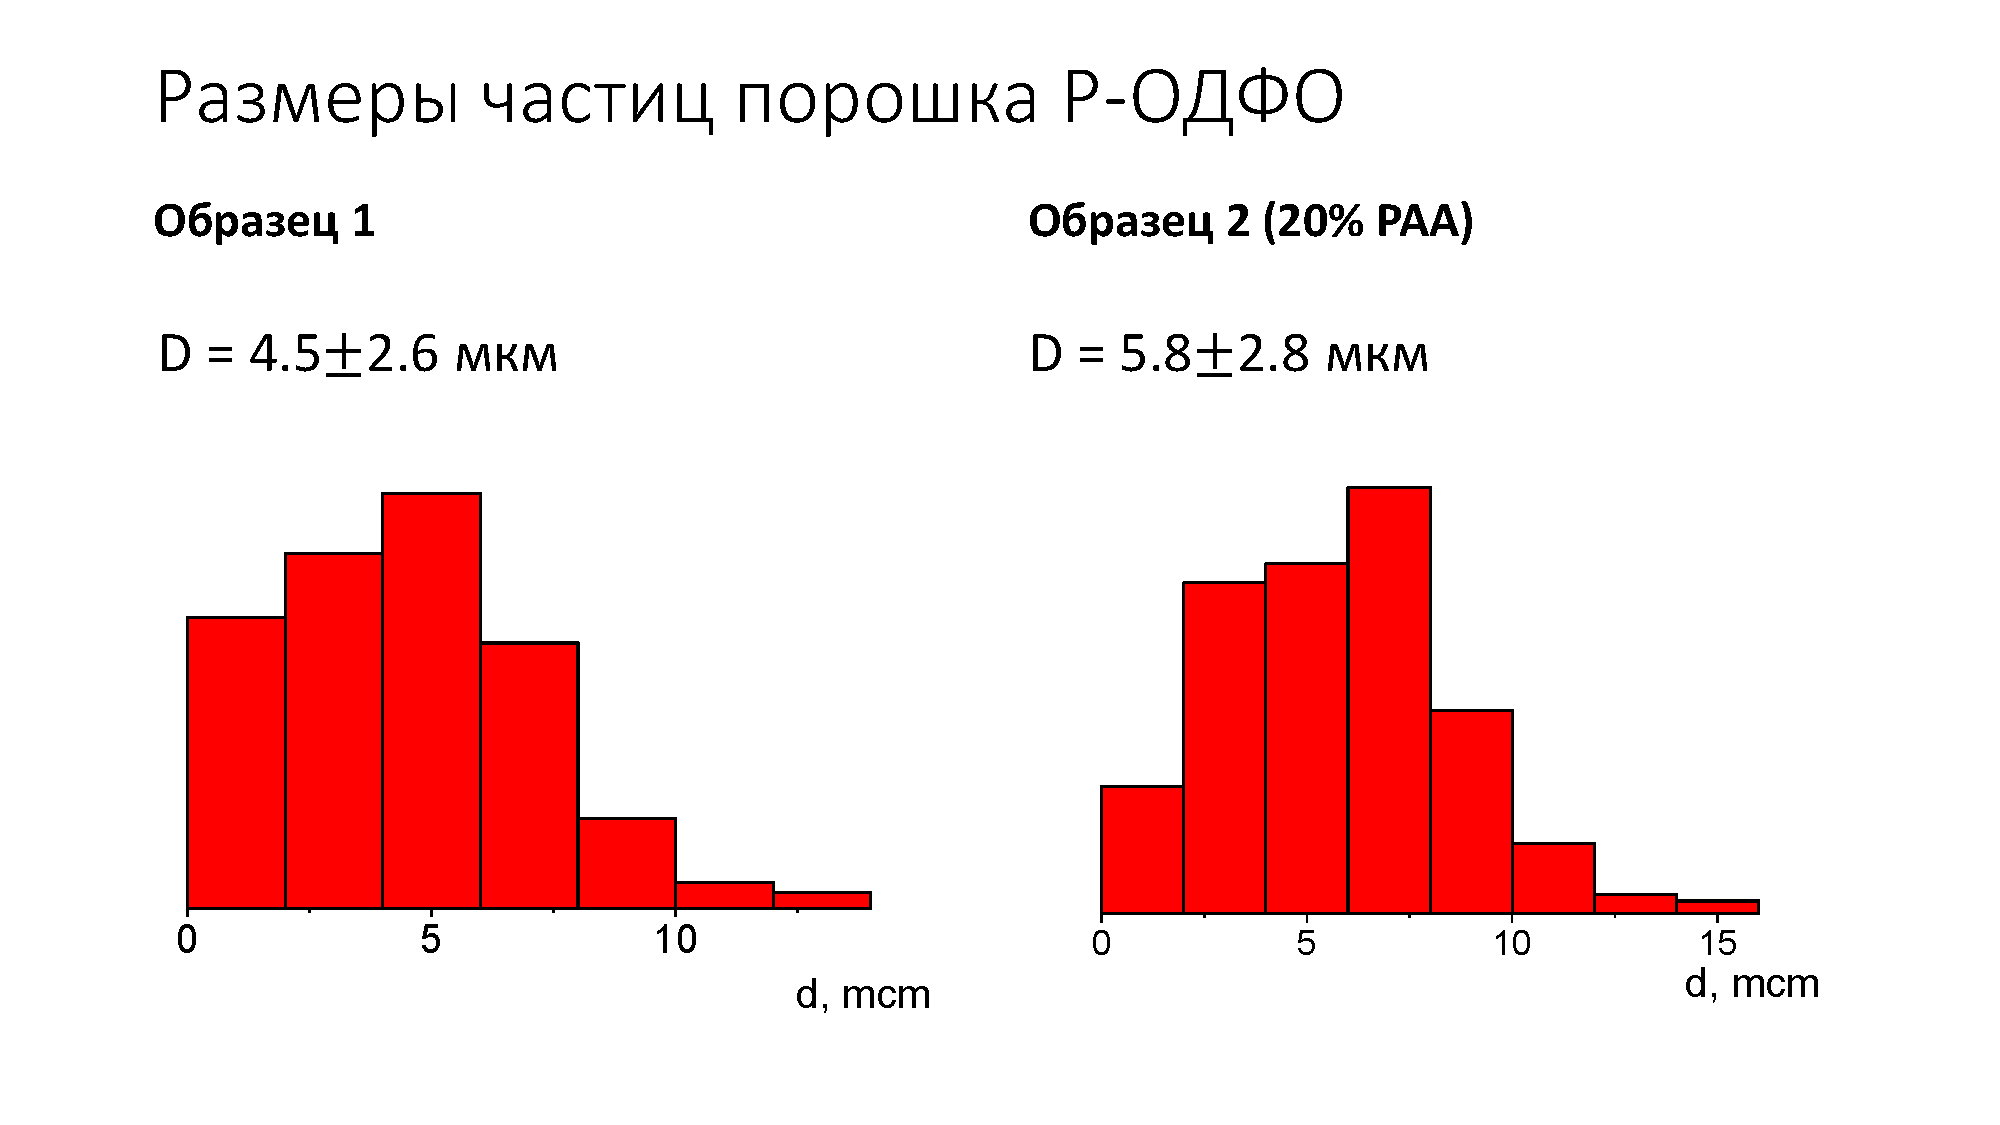
\includegraphics[width=\linewidth]{fig/particles}
	    \caption{Caption}
	    \label{fig:particles}
	\end{figure}
	
Измерения проводились на микрофокусной линии D13 Европейского центра синхротронного излучения (ERSF). Фото и схема ускоряющего кольца показаны на рис. \ref{fig:ring}. 
	
	
		\begin{figure}[h]\center
\begin{tabular}{cc}
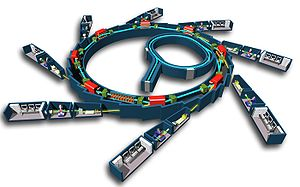
\includegraphics[width=0.5\linewidth]{fig/pribor-scheme.jpg}
&
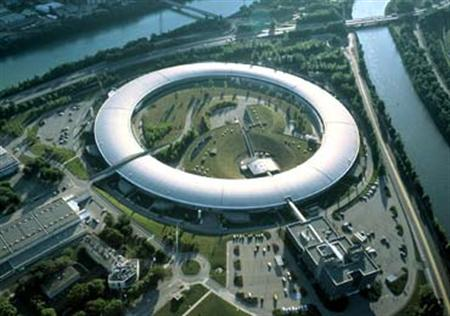
\includegraphics[width=0.5\linewidth]{fig/pribor-photo.jpg}
\end{tabular}
\caption{Синхротрон ERSF}
\label{fig:ring}
\end{figure}
	
А работает это так:
(тут еще картинка со схемой). Тогда получается большая интенсивность, бриллианс, статистика.



\section{Схема эксперимента}
Общая схема
Принципиальная схемаизображена на рис. \ref{fig:experiment}. 

\subsection{Источник}

\subsection{Детектор}

\subsection{Передвижение образца}


\begin{figure}[h]
    \centering
    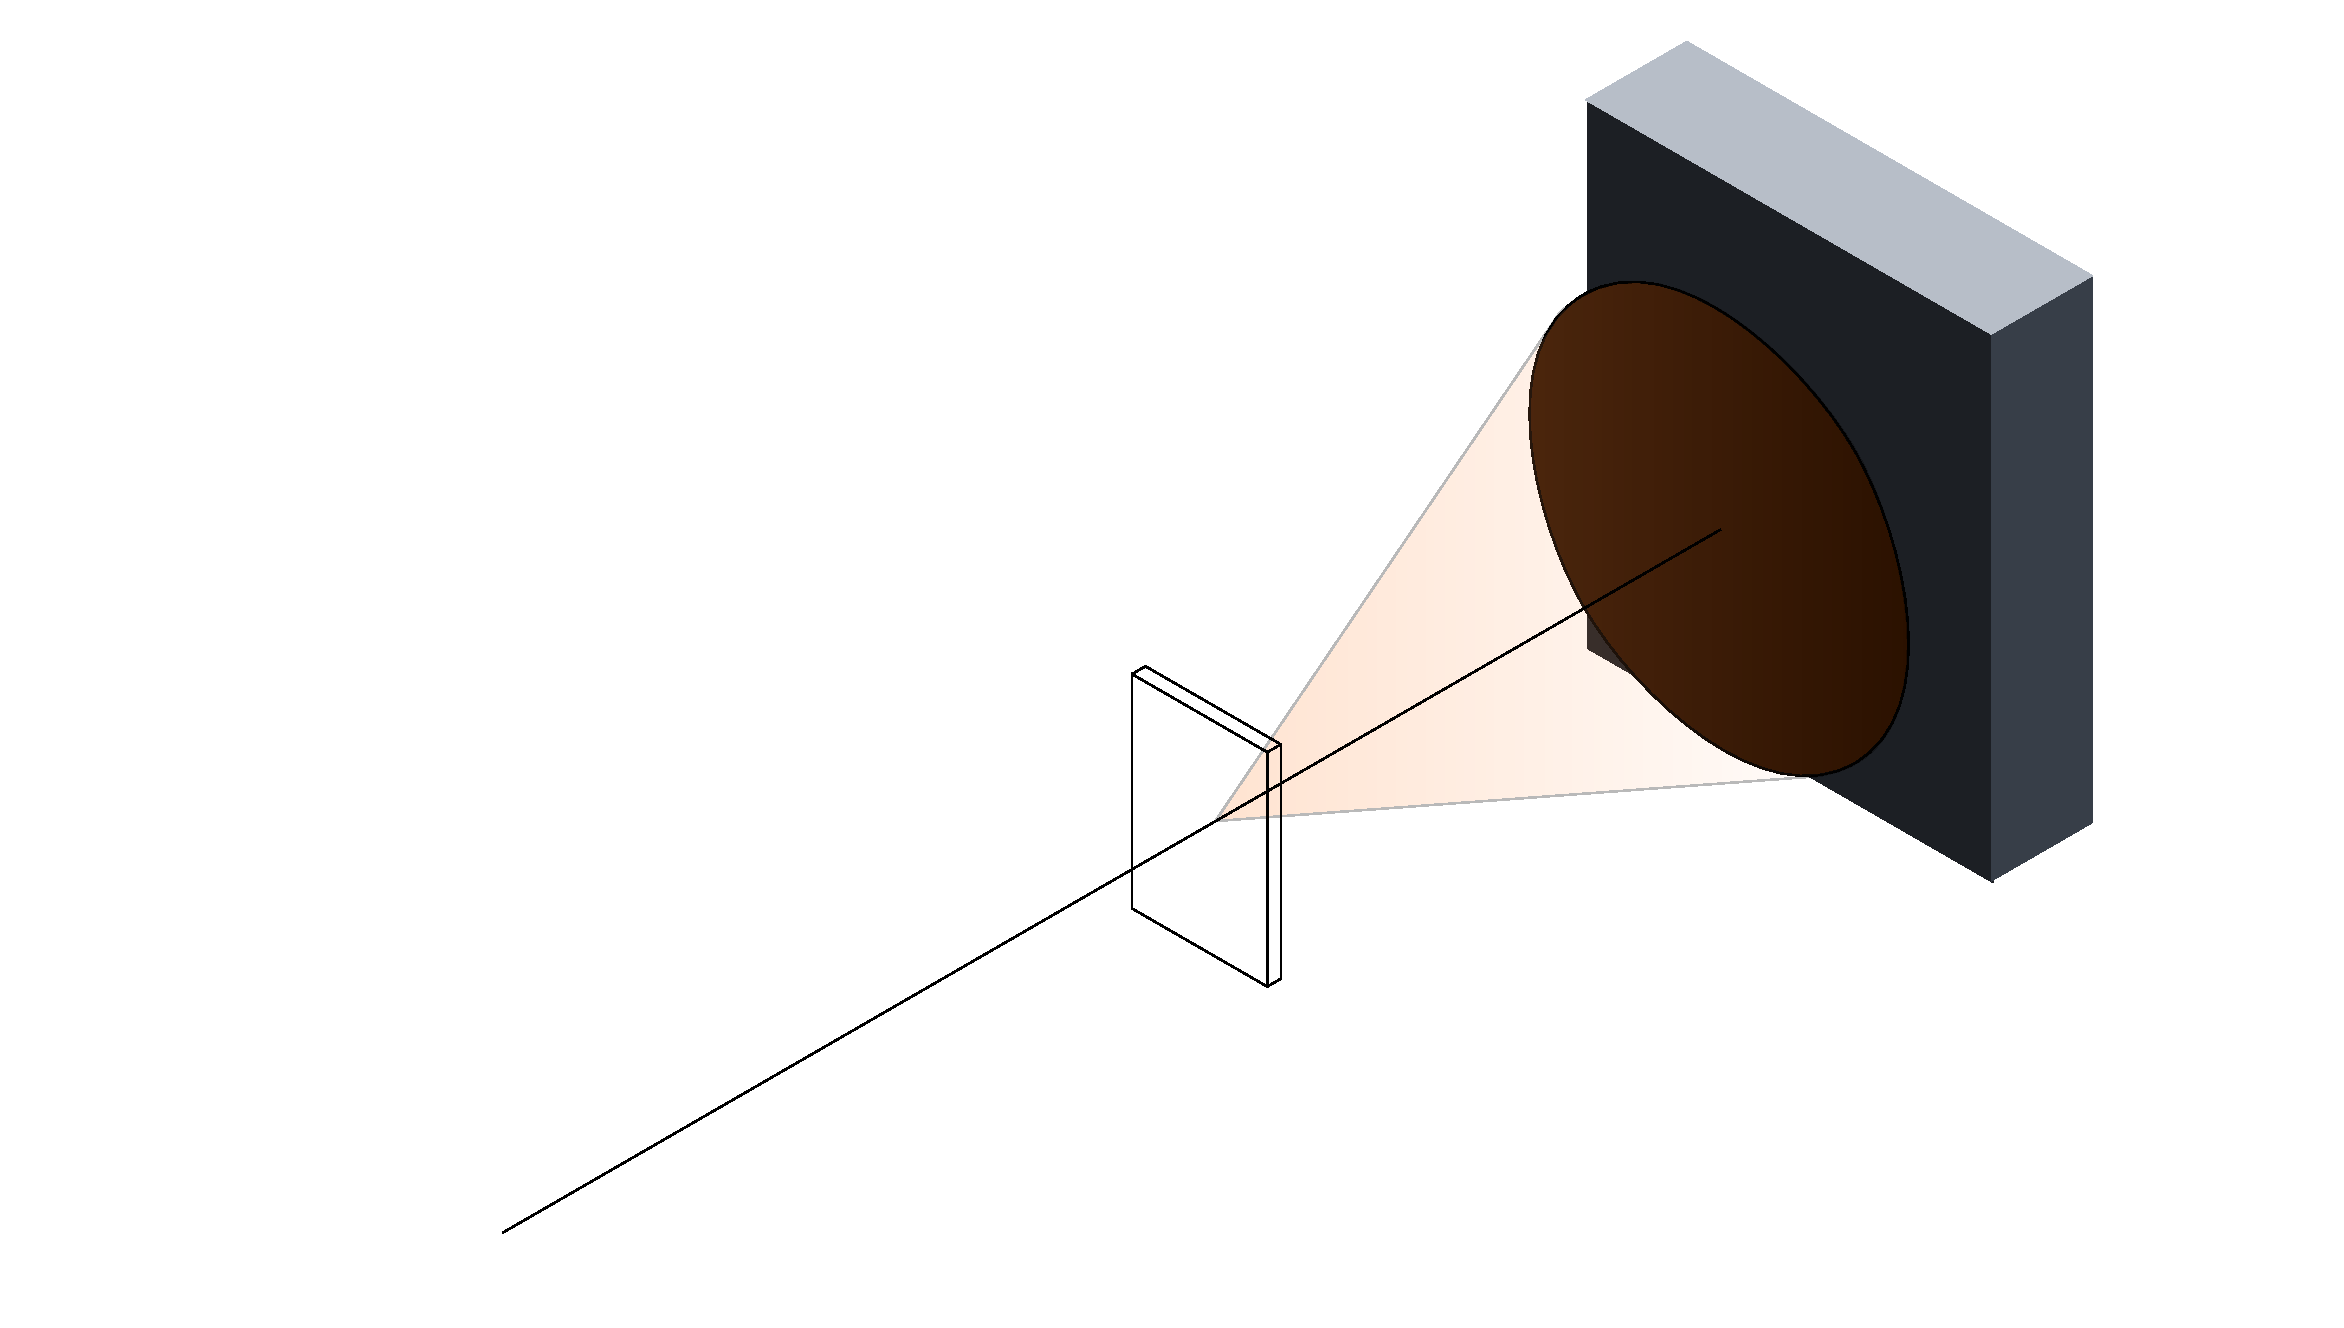
\includegraphics[width=\linewidth]{fig/experiment.pdf}
    \caption{[НЕ ДОРИСОВАНО] Схема эксперимента}
    \label{fig:experiment}
\end{figure}

\subsection{Калибровка}


 6.2.1 из 2д дифркции
 
 упомянуть про прочий подгон
 
Калибровка, а также азимутальное интегрирование производилось с помощью библиотеки pyFAI, \cite{pyfai}.



